\documentclass[10pt]{article}
\usepackage{enumitem}
\usepackage{amssymb}
\usepackage{amsmath}
\usepackage{geometry}
\usepackage{mathpazo}
\usepackage{microtype}

% --- TikZ Packages ---
\usepackage{tikz}
\usetikzlibrary{shapes, arrows.meta, positioning, fit, backgrounds, calc, decorations.pathreplacing, shadows}
% ---------------------

\geometry{margin=0.6in}
\setlength{\parskip}{0.5ex}
\setlength{\parindent}{0pt}
\setlist{leftmargin=*, nosep, before=\vspace{-0.5ex}, after=\vspace{0.5ex}}
\setlist[itemize]{leftmargin=1.5em}
\setlist[enumerate]{leftmargin=2em}

\title{Systemisation of Knowledge: Digital Liquidity}
\date{}

\begin{document}
\maketitle
\vspace{-1.5em}

\noindent\textit{This document is a planning outline for the first of four papers in a PhD thesis on digital liquidity. It establishes the foundational framework—the Balance-State Transition Event (BSTE) model and Digital Liquidity Stack—that underpins the three subsequent papers, which are described in Section~\ref{sec:subsequent}.}

\vspace{0.8em}

\section{Purpose and Positioning}

\subsection{High-Level Aims}

A unified, event-centric framework for
\emph{digital liquidity} across both legacy and tokenised infrastructures.

\begin{itemize}[noitemsep]
  \item Provide a \textbf{minimal, machine-checkable event model} (Balance-State Transition Event (BSTE)) for balance-state transitions.
  \item Define a \textbf{Digital Liquidity Stack} that captures money nature, ledger technology, clearing, settlement, finality, credit, encumbrance, and interoperability.
  \item Use this to systematically classify payment systems, Financial Market Infrastructures (FMIs), and tokenised systems (Real-Time Gross Settlement (RTGS), Automated Clearing House (ACH) / Deferred Net Settlement (DNS), card schemes, Continuous Linked Settlement (CLS), Central Counterparty (CCP) cash, stablecoins, Central Bank Digital Currencies (CBDCs), bridges, Automated Market Makers (AMMs), unified ledgers).
  \item Surface \textbf{patterns and failure modes} in digital liquidity management.
\end{itemize}

\subsection{Meaning of ``Digital Liquidity''}

Liqudity has multiple meanings:

\begin{enumerate}[label=(\alph*), noitemsep]
  \item \textbf{Market liquidity}: order-book depth, bid--ask spreads, price impact, AMM slippage.
  \item \textbf{Funding and settlement liquidity}: ability of institutions and infrastructures to obtain and deploy cash/collateral to meet obligations on time.
\end{enumerate}

In this work:

\begin{quote}
\textbf{Digital liquidity} means the \emph{capacity of digital infrastructures and participants to execute balance-state transitions} (our BSTEs)---to make obligations good in the right asset, on the right ledger, at the right time.
\end{quote}

We \emph{explicitly} do \textbf{not} attempt to survey or systematise market microstructure (order books, AMM curve design, price impact).
Those questions are treated as upper-layer phenomena and will be the subject of subsequent work.

\subsection{Intended Contributions}

The chapter / article delivers:

\begin{enumerate}[label=(C\arabic*), leftmargin=2cm]
  \item \textbf{BSTE model}: a minimal, compositional event representation for digital value movements.
  \item \textbf{Digital Liquidity Stack}: a 10-dimension core classification plus extended attributes to locate any system in a design space.
  \item \textbf{Mechanism taxonomy}: a systematic description of holds, locks, collateralisation, credit, queues, netting, Liquidity Savings Mechanisms (LSM), Payment versus Payment (PvP) / Delivery versus Payment (DvP) / Payment on Payment (PoP), channels, and bridges as compositions of BSTEs.
  \item \textbf{Comparative mapping}: worked classifications of representative legacy rails and tokenised systems.
  \item \textbf{Research agenda}: a bridge from this plumbing-level Systematization of Knowledge (SoK) to (i) formal optimisation (Paper~2) and (ii) empirical market stylised facts (Paper~3).
\end{enumerate}

\section{Scope of Background Review}

The following topics are in scope:

\begin{itemize}
  \item Classical payment systems and FMI literature:
    \begin{itemize}[noitemsep]
      \item RTGS design, LSM and gridlock-resolution algorithms.
      \item ACH/DNS systems, netting, risk management.
      \item CCPs and CLS (PvP systems), liquidity implications.
    \end{itemize}
  \item CBDC and unified-ledger architecture papers.
  \item Stablecoins, tokenised deposits, and tokenised collateral networks.
  \item Decentralized Finance (DeFi) systems: AMMs, lending protocols, cross-chain bridges.
  \item Existing ``stacks'' or taxonomies (e.g., generic blockchain stacks, CBDC design taxonomies).
  \item SoK methodology references (how SoK papers are typically structured).
\end{itemize}

The focus is \textbf{not} on exhaustive survey, but on situating this work among:
\begin{itemize}[noitemsep]
  \item payment/FMI engineering,
  \item tokenisation / Distributed Ledger Technology (DLT) infrastructure,
  \item SoK literature on distributed systems and crypto.
\end{itemize}

\section{BSTE: Balance-State Transition Event}

\subsection{Economic Owner Abstraction}

Introduce a conceptual mapping:
\[
  \mathrm{econ\_owner}(account) \to \text{beneficial owner (bank, customer, CCP, etc.)} .
\]

This allows us to distinguish:

\begin{itemize}[noitemsep]
  \item movements that change who owns the claim,
  \item movements that only change how an owner's claim is encumbered.
\end{itemize}

\subsection{Primitive Event Types}

\subsubsection*{Primitive P1: OWNERSHIP\_TRANSFER}

\begin{itemize}
  \item Economic owner multiset changes.
  \item Supply $S$ on the ledger is unchanged.
  \item Examples:
    \begin{itemize}[noitemsep]
      \item RTGS credit from bank A to bank B.
      \item On-chain Ethereum Request for Comments 20 (ERC20) token transfer.
      \item AMM swap legs where users receive tokens and AMM pool balances change.
    \end{itemize}
\end{itemize}

\subsubsection*{Primitive P2: ENCUMBRANCE\_ADJUST}

\begin{itemize}
  \item Economic owner set \emph{unchanged}, but claims move between:
    \begin{itemize}[noitemsep]
      \item free balance (\texttt{available}),
      \item encumbered buckets (holds, collateral, escrow, channels, etc.).
    \end{itemize}
  \item Constraint: $\mathrm{econ\_owner}(\mathrm{src\_account}) = \mathrm{econ\_owner}(\mathrm{dst\_account})$.
  \item Examples:
    \begin{itemize}[noitemsep]
      \item Card pre-authorisation: available $\to$ reservation.
      \item Central bank collateralisation: available $\to$ collateral.
      \item Hashed Time-Locked Contract (HTLC) lock: available $\to$ channel or bridge\_lock.
      \item Release of a hold: reservation $\to$ available.
    \end{itemize}
\end{itemize}

\subsubsection*{Primitive P3: SUPPLY\_ADJUST}

\begin{itemize}
  \item Net change in recognised supply $S$.
  \item Exactly one of \verb|src_account|, \verb|dst_account| equals
        \verb|EXTERNAL_SOURCE| or \verb|EXTERNAL_SINK|.
  \item Examples:
    \begin{itemize}[noitemsep]
      \item Central bank monetary operations in reserves.
      \item Stablecoin mint/burn.
      \item Protocol base-fee burn.
    \end{itemize}
\end{itemize}

% --- DIAGRAM 1: BSTE PRIMITIVES ---
\begin{figure}[h]
    \centering
    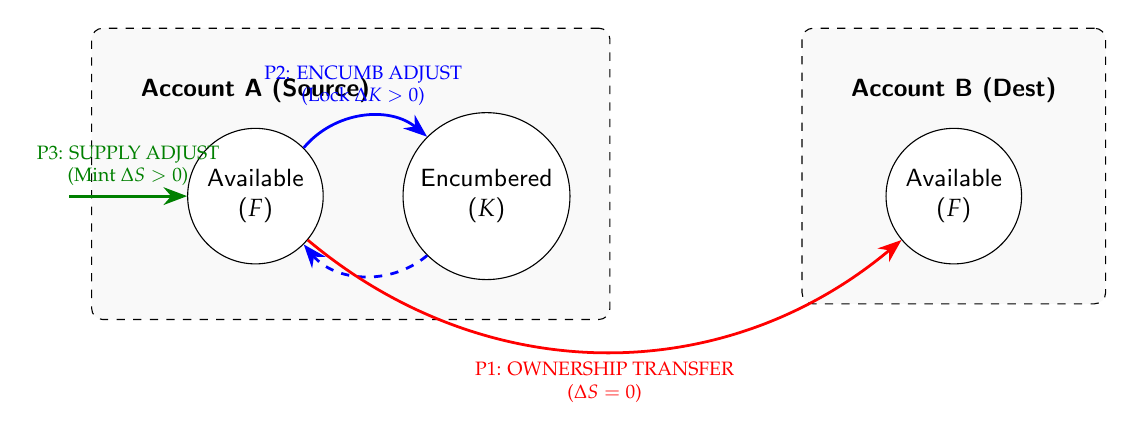
\begin{tikzpicture}[
        node distance=1.5cm,
        account/.style={draw, rounded corners, inner sep=0.5cm, fill=gray!5, dashed},
        bucket/.style={circle, draw, minimum size=1.5cm, fill=white, align=center, font=\sffamily\small},
        op_arrow/.style={->, >={Stealth[length=3mm]}, line width=1pt},
        label_text/.style={font=\sffamily\bfseries\small}
    ]

    % --- Account A (Source) ---
    \node[bucket] (a_avail) {Available\\($F$)};
    \node[bucket, right=1.0cm of a_avail] (a_lock) {Encumbered\\($K$)};
    \node[label_text, above=0.2cm of a_avail] (lbl_a) {Account A (Source)};

    % Draw Account A Box
    \begin{scope}[on background layer]
        \node[account, fit=(a_avail) (a_lock) (lbl_a)] (box_a) {};
    \end{scope}

    % --- Account B (Dest) ---
    \node[bucket, right=4.0cm of a_lock] (b_avail) {Available\\($F$)};
    \node[label_text, above=0.2cm of b_avail] (lbl_b) {Account B (Dest)};

    % Draw Account B Box
    \begin{scope}[on background layer]
        \node[account, fit=(b_avail) (lbl_b)] (box_b) {};
    \end{scope}

    % --- Operations ---

    % 1. Encumbrance Adjust (P2)
    \draw[op_arrow, blue] (a_avail) to[bend left=45] node[midway, above, font=\scriptsize, align=center, text=blue] {P2: ENCUMB ADJUST\\(Lock $\Delta K > 0$)} (a_lock);
    \draw[op_arrow, blue, dashed] (a_lock) to[bend left=45] (a_avail);

    % 2. Ownership Transfer (P1)
    \draw[op_arrow, red] (a_avail) to[out=320, in=220] node[midway, below, font=\scriptsize, align=center, text=red] {P1: OWNERSHIP TRANSFER\\($\Delta S = 0$)} (b_avail);

    % 3. Supply Adjust (P3)
    \node[left=1.5cm of a_avail] (void) {};
    \draw[op_arrow, green!50!black] (void) -- node[midway, above, font=\scriptsize, align=center, text=green!50!black] {P3: SUPPLY ADJUST\\(Mint $\Delta S > 0$)} (a_avail);

    \end{tikzpicture}
    \caption{The Three Kernel Primitives of the BSTE Model. All digital value movement is composed of these atomic transitions between Free ($F$) and Encumbered ($K$) sub-balances, or between ledgers/the external system.}
\end{figure}
% ---------------------------------

\subsection{Canonical BSTE Schema}

We adopt the following design choices:

\begin{itemize}[noitemsep]
  \item \verb|amount| is strictly positive.
  \item No structural \texttt{NULL}; use explicit sentinels.
  \item Encumbrance is derived from bucket types; no \verb|lock_delta|.
\end{itemize}

\subsubsection*{Identity and Ordering}

\begin{enumerate}[label=\arabic*.]
  \item \verb|event_id| : unique identifier.
  \item \verb|ledger_id| : authoritative balance-record; may be Central Bank (CB) RTGS, bank core, scheme settlement file, or DLT state machine.
  \item \verb|asset_code| : identifies the asset.
  \item \verb|op_kind| : \{OWNERSHIP\_TRANSFER, ENCUMBRANCE\_ADJUST, SUPPLY\_ADJUST\}.
  \item \verb|t_occurred| : logical posting time.
  \item \verb|event_seq| : per-ledger total order index.
\end{enumerate}

\subsubsection*{Accounts and Balance Types}

\begin{enumerate}[label=\arabic*.]
  \setcounter{enumi}{6}
  \item \verb|src_account| : string, or \verb|EXTERNAL_SOURCE|.
  \item \verb|src_balance_type| : \{available, reservation, collateral, escrow, channel, internal\_pending, bridge\_lock, other\}.
  \item \verb|dst_account| : string, or \verb|EXTERNAL_SINK|.
  \item \verb|dst_balance_type| : same enum.
\end{enumerate}

Encumbered buckets are those with \verb|balance_type| $\neq$ \texttt{available} (but we may specify the exact list).

\subsubsection*{Supply and Economic Role}

\begin{enumerate}[label=\arabic*.]
  \setcounter{enumi}{10}
  \item \verb|supply_delta| : signed change to supply on the ledger.
  \item \verb|economic_role| : \{principal, fee, tax, interest, margin, collateral\_movement, other\}.
  \item \verb|tax_subtype| : optional detail for \texttt{economic\_role = tax}.
\end{enumerate}

All fees/taxes are represented as ordinary BSTEs with appropriate \verb|economic_role|.

\subsubsection*{Grouping and Atomic Sets}

\begin{enumerate}[label=\arabic*.]
  \setcounter{enumi}{13}
  \item \verb|group_id| : business group (Foreign Exchange (FX) trade, batch, clearing cycle).
  \item \verb|link_id| : groups events into an atomic or quasi-atomic set.
\end{enumerate}

Atomic semantics are kept in a separate table \texttt{atomic\_sets}, keyed by \verb|link_id|, with fields:

\begin{itemize}[noitemsep]
  \item \verb|atomic_pattern| : none, PvP, DvP, PoP.
  \item \verb|atomic_mechanism| : single\_ledger\_tx, central\_novation, htlc, escrow\_agent, optimistic\_with\_fraud\_proof, trusted\_coordinator.
  \item \verb|atomic_params| : JSON (timeout heights, hashlocks, etc.).
  \item \verb|fx_rate| and \verb|price_reference| : optional for cross-asset sets.
\end{itemize}

\subsubsection*{Evidence, Expiry, Notes}

\begin{enumerate}[label=\arabic*.]
  \setcounter{enumi}{16}
  \item \verb|message_ref| : upstream messages/logs (International Organization for Standardization (ISO) 20022 financial messages, ISO 8583 card transaction messages, transaction hashes).
  \item \verb|purpose_code| : business purpose.
  \item \verb|expiry_time| : for encumbrances with timeouts (HTLCs, auth holds, etc.).
  \item \verb|notes| : free text.
\end{enumerate}

\section{Pending Events}

Introduce Pending-BSTE (Pending Balance-State Transition Event (PBSTE)) as an operational extension:

\begin{itemize}
  \item Structural fields mirror BSTE.
  \item Additional fields:
    \begin{itemize}[noitemsep]
      \item \verb|t_proposed|,
      \item \verb|status| $\in$ \{pending, accepted, rejected, cancelled\}.
    \end{itemize}
\end{itemize}

PBSTEs do not affect:
\begin{itemize}[noitemsep]
  \item supply $S(t)$,
  \item encumbrance $K(t)$,
  \item free balances in the canonical historical accounting.
\end{itemize}

They do affect projected liquidity:
\[
  F_{\mathrm{projected}}(t)
  = F_{\mathrm{posted}}(t)
    - \sum_{\text{pending outflows}} \mathrm{amount} .
\]

\section{Global Invariants and Bridging Semantics}

\subsection{Per-Ledger Supply and Encumbrance}

For each (\texttt{ledger\_id}, \texttt{asset\_code}):

\begin{itemize}
  \item Supply:
    \[
      S(t) = S(t_0) + \sum_{\text{events }\le t} \mathrm{supply\_delta} .
    \]
  \item Encumbered quantity:
    \[
      K(t) = \sum_{\text{accounts, encumbered buckets}} \mathrm{balance}(t) .
    \]
  \item Free balance per account:
    \[
      \mathrm{FreeBalance}(t) \ge 0.
    \]
\end{itemize}

\subsection{Primitive-Level Constraints}

\begin{itemize}[noitemsep]
  \item \textbf{P1 OWNERSHIP\_TRANSFER}: \verb|supply_delta = 0|.
  \item \textbf{P2 ENCUMBRANCE\_ADJUST}: \verb|supply_delta = 0| and
        $\mathrm{econ\_owner}(\mathrm{src}) = \mathrm{econ\_owner}(\mathrm{dst})$.
  \item \textbf{P3 SUPPLY\_ADJUST}: exactly one endpoint is external.
\end{itemize}

\subsection{Atomic Sets}

For each \verb|link_id|, there is an entry in \texttt{atomic\_sets} describing the intended pattern and mechanism.

Invariants include:

\begin{itemize}[noitemsep]
  \item For PvP: no leg should settle in isolation (interpretation depends on mechanism).
  \item For DvP: cash and security legs are coupled.
  \item For HTLCs: encumbrances must be released by either success or timeout.
\end{itemize}

\subsection{Bridging Invariants}

For lock-and-mint bridges:

\begin{itemize}
  \item Backing ledger uses \verb|bridge_lock| buckets for locked units.
  \item Wrapped asset ledger mints new tokens via \textbf{SUPPLY\_ADJUST}.
\end{itemize}

A simple invariant for one-to-one lock-mint:

\[
  S_{\mathrm{wrapped}}(t) \le K_{\mathrm{backing, bridge\_lock}}(t)
\]
(equality up to fees/slippage).

% --- DIAGRAM 4: BRIDGING INVARIANTS ---
\begin{figure}[h]
    \centering
    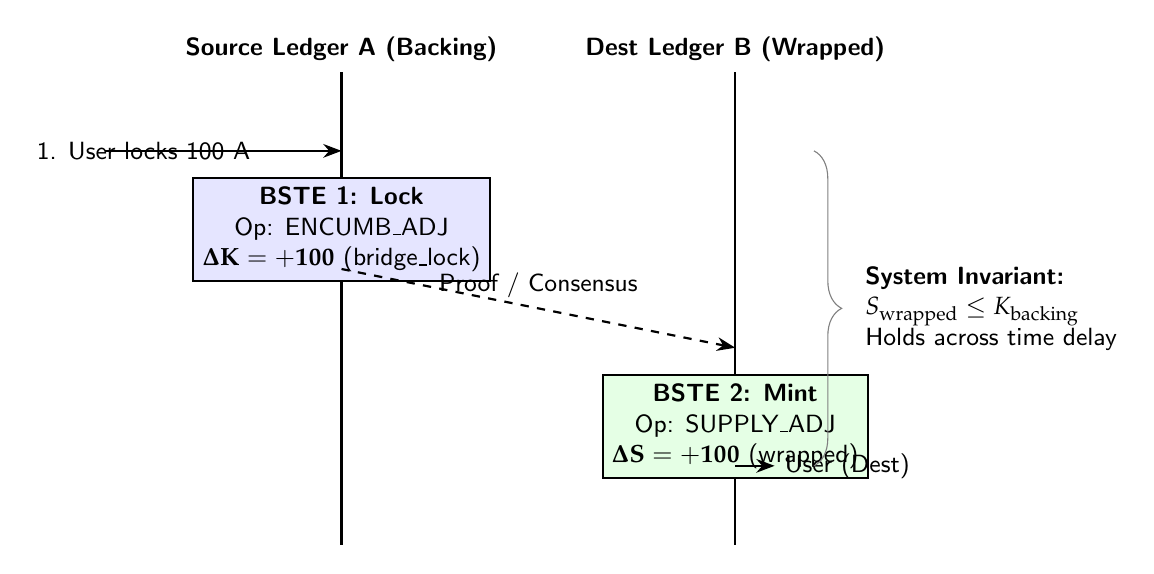
\begin{tikzpicture}[
        font=\sffamily\small,
        thick,
        >=Stealth
    ]

    % Lifelines
    \draw (3,0) node[above] {\textbf{Source Ledger A (Backing)}} -- (3,-6);
    \draw (8,0) node[above] {\textbf{Dest Ledger B (Wrapped)}} -- (8,-6);

    % Time T1: Lock on Source (BSTE 1)
    \node[anchor=west] at (-1, -1) {1. User locks 100 A};
    \draw[->] (0,-1) -- (3,-1);

    % BSTE Event: Lock
    \node[draw, fill=blue!10, align=center, minimum width=2.5cm] at (3, -2) {
        \textbf{BSTE 1: Lock}\\
        Op: ENCUMB\_ADJ\\
        $\mathbf{\Delta K = +100}$ (bridge\_lock)
    };

    % Message Passing (Relayer/Proof)
    \draw[->, dashed, line width=0.8pt] (3,-2.5) -- node[midway, above] {Proof / Consensus} (8,-3.5);

    % BSTE Event: Mint
    \node[draw, fill=green!10, align=center, minimum width=2.5cm] at (8, -4.5) {
        \textbf{BSTE 2: Mint}\\
        Op: SUPPLY\_ADJ\\
        $\mathbf{\Delta S = +100}$ (wrapped)
    };

    % Time T2: Credit User
    \draw[->] (8,-5) -- (8.5,-5) node[right] {User (Dest)};

    % Invariant Annotation
    \draw[decorate, decoration={brace, amplitude=10pt}, thin, gray] (9,-1) -- (9,-5)
        node[midway, right=15pt, align=left, text=black] {
            \textbf{System Invariant:}\\
            $S_{\mathrm{wrapped}} \le K_{\mathrm{backing}}$\\
            Holds across time delay
        };

    \end{tikzpicture}
    \caption{BSTE Sequence for Lock-and-Mint Bridging. The increase in $S$ on the destination ledger is matched by an increase in $K$ (Encumbrance) on the source ledger, ensuring the global free quantity remains conserved.}
\end{figure}
% -----------------------------------

\section{Digital Liquidity Stack (Core and Extended)}

\subsection{Core Dimensions}

These are the 10 core fields used for classification tables.

% --- DIAGRAM 2: DIGITAL LIQUIDITY STACK ---
\begin{figure}[h]
    \centering
    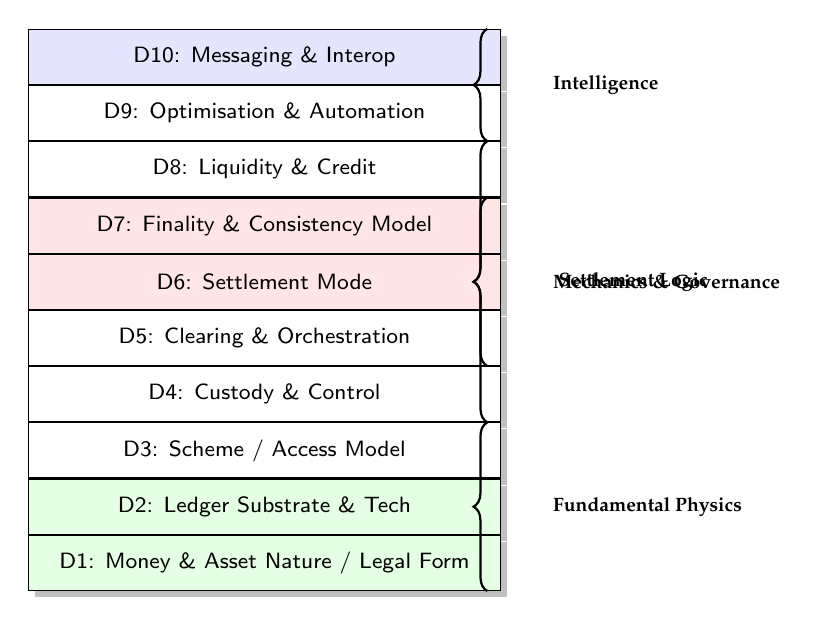
\begin{tikzpicture}[
        layer_box/.style={
            draw, rectangle, minimum width=6cm, minimum height=0.7cm,
            align=center, font=\sffamily\footnotesize, fill=white, drop shadow
        },
        group_brace/.style={
            decorate, decoration={brace, amplitude=5pt, mirror, raise=5pt}, thick
        }
    ]

    % Define the layers (Bottom to Top)
    \node[layer_box, fill=blue!10] (L10) {D10: Messaging \& Interop};
    \node[layer_box, below=0cm of L10] (L9) {D9: Optimisation \& Automation};
    \node[layer_box, below=0cm of L9] (L8) {D8: Liquidity \& Credit};
    \node[layer_box, below=0cm of L8, fill=red!10] (L7) {D7: Finality \& Consistency Model};
    \node[layer_box, below=0cm of L7, fill=red!10] (L6) {D6: Settlement Mode};
    \node[layer_box, below=0cm of L6] (L5) {D5: Clearing \& Orchestration};
    \node[layer_box, below=0cm of L5] (L4) {D4: Custody \& Control};
    \node[layer_box, below=0cm of L4] (L3) {D3: Scheme / Access Model};
    \node[layer_box, below=0cm of L3, fill=green!10] (L2) {D2: Ledger Substrate \& Tech};
    \node[layer_box, below=0cm of L2, fill=green!10] (L1) {D1: Money \& Asset Nature / Legal Form};

    % Groupings (Braces)
    \draw[group_brace] (L10.north east) -- (L9.south east) node[midway, right=15pt, font=\bfseries\scriptsize] {Intelligence};
    \draw[group_brace] (L8.north east) -- (L4.south east) node[midway, right=15pt, font=\bfseries\scriptsize] {Mechanics \& Governance};
    \draw[group_brace] (L7.north east) -- (L5.south east) node[midway, right=15pt, font=\bfseries\scriptsize, xshift=2pt] {Settlement Logic};
    \draw[group_brace] (L3.north east) -- (L1.south east) node[midway, right=15pt, font=\bfseries\scriptsize] {Fundamental Physics};

    \end{tikzpicture}
    \caption{The Digital Liquidity Stack (10 Core Dimensions). Each system/asset is located by a coordinate in this design space.}
\end{figure}
% ---------------------------------

\begin{enumerate}[label=\textbf{D\arabic*}.]
  \item \textbf{asset\_nature}:
    cb\_reserve, cb\_cash, commercial\_deposit, e\_money, stablecoin\_fiat,
    stablecoin\_crypto, token\_native, security\_cash, other.
  \item \textbf{legal\_form}:
    balance\_sheet\_claim, trust\_unit, fund\_share, bearer\_instrument,
    synthetic\_derivative, cb\_direct.
  \item \textbf{representation\_model}:
    native\_account, native\_token, wrapped\_mirror, synthetic.
  \item \textbf{ledger\_tech}:
    cb\_rtgs, bank\_core, ccp\_cash\_ledger, cls\_pvp,
    dlt\_public, dlt\_permissioned, scheme\_internal, channel\_state, other.
  \item \textbf{account\_model}:
    account\_balances, Unspent Transaction Output (utxo), smart\_contract\_state, hybrid.
  \item \textbf{scheme\_type}:
    rtgs\_operator, instant\_payments, ach\_dns, card\_scheme,
    correspondent\_network, Decentralized Exchange (dex)\_protocol, bridge\_protocol,
    mobile\_money\_scheme, other.
  \item \textbf{access\_model}:
    direct, indirect, retail, wholesale, permissionless, permissioned.
  \item \textbf{clearing\_mechanism}:
    none\_gross, bilateral\_net, multilateral\_net, queue\_lsm,
    continuous\_net, offchain\_channels.
  \item \textbf{settlement\_mode}:
    gross, bilateral\_net\_batch, multilateral\_net\_batch,
    hybrid\_queue\_lsm, onchain\_gross, onchain\_batch.
  \item \textbf{finality\_kind} and \textbf{consistency\_model}:
    deterministic / deterministic\_deferred / probabilistic vs
    eventual\_reconciliation / consensus\_atomic / hybrid.
\end{enumerate}

\subsection{Extended Dimensions}

Extended fields that can be used in deeper analysis or thesis-only tables:

\begin{itemize}
  \item custody\_model, authorisation\_model, freeze\_authority.
  \item credit\_sources, encumbrance\_eligibility, allows\_negative\_balances.
  \item optimisation\_style, optimisation\_scope.
  \item messaging\_standards, addressing\_scheme, id\_scheme.
  \item privacy\_model, replay\_guard.
  \item governance\_model, legal\_finality\_basis.
\end{itemize}

\section{Tokenised vs Non-Tokenised vs Hybrid}

\subsection{Non-Tokenised Systems}

Common characteristics:

\begin{itemize}[noitemsep]
  \item representation\_model = native\_account,
  \item ledger\_tech = cb\_rtgs / bank\_core / scheme\_internal,
  \item consistency\_model = eventual\_reconciliation,
  \item execution is message-driven, core state is opaque during processing.
\end{itemize}

\subsection{Tokenised Systems}

Common characteristics:

\begin{itemize}[noitemsep]
  \item representation\_model $\in$ \{native\_token, wrapped\_mirror\},
  \item ledger\_tech = dlt\_public or dlt\_permissioned,
  \item consistency\_model = consensus\_atomic,
  \item programmability: smart contracts see state and update in the same transaction.
\end{itemize}

\subsection{Hybrid Systems}

Examples:

\begin{itemize}[noitemsep]
  \item Tokenised deposits that sit atop bank cores but expose a token interface.
  \item RLN / unified-ledger designs with central-bank and commercial-bank tiers.
  \item Card schemes or Payment Service Providers (PSPs) that mirror balances onto a DLT sub-ledger.
\end{itemize}

Discussion will emphasise:
\begin{itemize}[noitemsep]
  \item how hybrid systems occupy intermediate coordinates in the stack,
  \item distinct failure modes and liquidity behaviours.
\end{itemize}

\section{Taxonomy of Liquidity Mechanisms}

This section classifies mechanisms as compositions of BSTEs at specific stack coordinates.

\subsection{Credit and Funding}

\begin{itemize}[noitemsep]
  \item Intraday central-bank credit (RTGS).
  \item Overdrafts and bilateral credit lines.
  \item Repo-based liquidity provision.
\end{itemize}

\subsection{Encumbrances and Collateral}

\begin{itemize}[noitemsep]
  \item Holds (card, instant payments).
  \item CCP margin and haircuts.
  \item Collateralisation at central bank / CCP / DLT-based vaults.
\end{itemize}

\subsection{Clearing and Netting}

\begin{itemize}[noitemsep]
  \item Bilateral and multilateral netting.
  \item LSM / gridlock resolution.
  \item DNS transfer cycles and settlement windows.
\end{itemize}

% --- DIAGRAM 3: LIQUIDITY TOPOLOGIES ---
\begin{figure}[h]
    \centering
    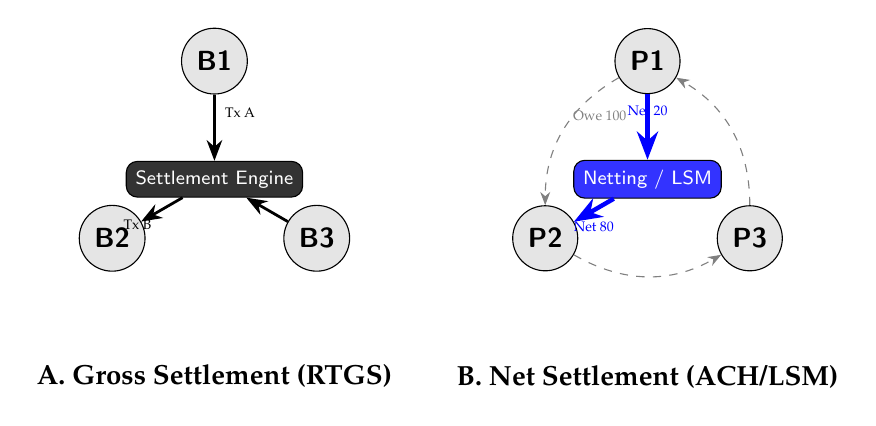
\begin{tikzpicture}[
        node distance=1.5cm,
        participant/.style={circle, draw, fill=gray!20, minimum size=0.8cm, font=\sffamily\bfseries},
        center_node/.style={rectangle, draw, fill=black!80, text=white, rounded corners, font=\sffamily\scriptsize},
        flow/.style={->, >={Stealth}, line width=1pt, black},
        obligation/.style={->, >={Stealth}, dashed, gray},
        net_flow/.style={->, >={Stealth}, ultra thick, blue}
    ]

    % --- Left: Gross Settlement (Star) ---
    \node[center_node] (rtgs) at (0,0) {Settlement Engine};
    \node[participant] (b1) at (90:1.5) {B1};
    \node[participant] (b2) at (210:1.5) {B2};
    \node[participant] (b3) at (330:1.5) {B3};

    \draw[flow] (b1) -- node[above right, font=\tiny] {Tx A} (rtgs);
    \draw[flow] (rtgs) -- node[below left, font=\tiny] {Tx B} (b2);
    \draw[flow] (b3) -- (rtgs);
    \node[below=2cm of rtgs, font=\bfseries] {A. Gross Settlement (RTGS)};

    % --- Right: Netting / LSM (Mesh) ---
    \begin{scope}[xshift=5.5cm]
        \node[center_node, fill=blue!80] (algo) at (0,0) {Netting / LSM};
        \node[participant] (p1) at (90:1.5) {P1};
        \node[participant] (p2) at (210:1.5) {P2};
        \node[participant] (p3) at (330:1.5) {P3};

        % Obligations (The problem)
        \draw[obligation] (p1) to[bend right] node[above right, font=\tiny] {Owe 100} (p2);
        \draw[obligation] (p2) to[bend right] (p3);
        \draw[obligation] (p3) to[bend right] (p1);

        % Net Settlement (The solution)
        \draw[net_flow] (p1) -- node[above, font=\tiny] {Net 20} (algo);
        \draw[net_flow] (algo) -- node[below, font=\tiny] {Net 80} (p2);

        \node[below=2cm of algo, font=\bfseries] {B. Net Settlement (ACH/LSM)};
    \end{scope}

    \end{tikzpicture}
    \caption{Liquidity Mechanism Topologies. Gross Settlement (A) requires flow equal to the full transaction value. Net Settlement (B) resolves obligations (dashed) into smaller, net flows (solid) via an aggregator, conserving liquidity.}
\end{figure}
% -----------------------------------

\subsection{Channels and Off-Chain Mechanisms}

\begin{itemize}[noitemsep]
  \item Payment channels (Lightning and analogues).
  \item State channels, rollups with periodic settlement.
\end{itemize}

\subsection{PvP, DvP, PoP, and Bridges}

\begin{itemize}[noitemsep]
  \item PvP FX legs across RTGS or DLTs.
  \item DvP securities settlement vs cash.
  \item PoP patterns where obligations are offset.
  \item Bridge designs: custodial lock-mint, burn-and-mint, synthetic representations.
\end{itemize}

\section{Representative Case Studies}

This section will contain 3--5 in-depth examples, each with:

\begin{itemize}[noitemsep]
  \item stack coordinates,
  \item BSTE sequences for typical flows,
  \item encumbrance and credit implications.
\end{itemize}

Candidate case studies:

\begin{enumerate}
  \item \textbf{Central-bank RTGS with LSM}.
        Show queued payments, LSM runs, BSTE-level effect.
  \item \textbf{Card scheme + DNS}.
        Auth holds, clearing batches, RTGS settlement, chargebacks.
  \item \textbf{Instant retail system (e.g., New Payments Platform (NPP)-like)}.
        Real-time credits with holds and CB RTGS backing.
  \item \textbf{DeFi AMM swap + cross-chain bridge}.
        Multi-leg on-chain bundles, HTLCs, finality and latency.
  \item \textbf{Tokenised deposit / unified ledger}.
        Hybrid consistency, legal form, governance.
\end{enumerate}

\section{Design Space and Discussion}

Here the chapter synthesises:

\begin{itemize}
  \item How different systems cluster in the 10-dimensional core space.
  \item Trade-offs:
    \begin{itemize}[noitemsep]
      \item pre-funded vs credit-backed,
      \item gross vs net settlement,
      \item centralised vs consensus-based finality,
      \item transparency vs privacy,
      \item simplicity vs programmability.
    \end{itemize}
  \item Failure modes:
    \begin{itemize}[noitemsep]
      \item reconciliation drift,
      \item reorg risk,
      \item stuck encumbrances (e.g., HTLC timeouts, unresolved holds),
      \item bridge misconfigurations and backing failures.
    \end{itemize}
\end{itemize}

This section also positions emerging designs (Regulated Liability Networks (RLN), unified ledgers, tokenised collateral networks) in the space.

\section{Subsequent Papers Overview}
\label{sec:subsequent}

\subsection{Stylised Facts of Tokenised Real World Asset Markets (Paper 2)}

Explain how:

\begin{itemize}[noitemsep]
  \item BSTE encoding allows uniform extraction of transaction and settlement data.
  \item Stack coordinates inform:
    \begin{itemize}[noitemsep]
      \item which systems are comparable,
      \item where latencies and failures originate.
    \end{itemize}
  \item Empirical stylised facts can then be tied explicitly to plumbing choices.
\end{itemize}

\subsection{Collateral as Settlement Asset (Paper 3)}

Show how:

\begin{itemize}[noitemsep]
  \item legal\_form, governance\_model, and encumbrance semantics in the stack
        become central to designing repo-native money and collateral tokens.
  \item invariants from the SoK constrain safe designs for yield-bearing settlement assets.
\end{itemize}

\subsection{Agentic Liquidity (Paper 4)}

Outline how the BSTE + stack model supports:

\begin{itemize}[noitemsep]
  \item Formal graph representations of multi-ledger liquidity.
  \item Problem statements of the form: \\
        ``Given required OWNERSHIP\_TRANSFER BSTEs,
        find ENCUMBRANCE\_ADJUST and routing decisions that minimise
        a cost functional such as $\int K(t)\, dt$ subject to constraints.''
  \item Integration of LSM/queueing, Mixed Integer Linear Programming (MILP) / Model Predictive Control (MPC), Reinforcement Learning (RL) agents.
\end{itemize}

\end{document}